\begin{example}\label{TEO:ex_CitDiveder01}
  V elektronických soustavách se největších přesností dosahuje u rezistorů, kde je standardně 
  zaručována chyba menší než 1\%, u přesných 0.1\% a u velmi přesných 0.01\%.

  \begin{figure}
   \centering
    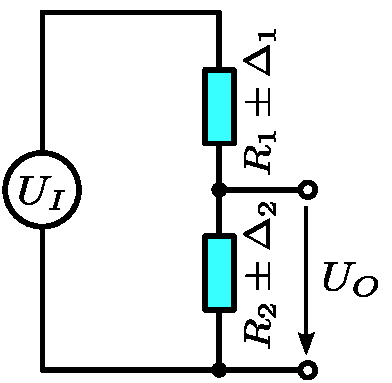
\includegraphics[width=0.4\linewidth]{voltage_divider.pdf}
    \caption{ }
    \label{TEO:fig_voltage_divider}
  \end{figure}

  Bude nás zajímat jaký vliv má tolerance rezistorů na výsledný poměr výstupního ku vstupnímu 
  napětí a také, zda-li při různě zvoleném poměru těchto rezistorů se bude měnit velikost chyby, 
  ačkoliv budou mít stejnou přesnost. Intuitivně předpokládáme, že  nejnepříznivější situace  
  nastane, když hodnoty použitých rezistorů padnou na opačné strany tolerančních pásem, jenž 
  reprezentuje $\Delta_1$ a $\Delta_2$ tj. $R_2 - \Delta_2R_2$ a $R_1 + \Delta_1R_1$ nebo $R_2 + 
  \Delta_2R_2$ a $R_1 - \Delta_1R_1$. V obou případech bude chyba stejná, proto si vybereme 
  například první případ a zapíšeme (rov. \ref{TEO:eq_divider_1}).
  \begin{equation}\label{TEO:eq_divider_1}
    \frac{U_o}{U_i} = \frac{R_2-\Delta_2 R_2}{R_1+\Delta_1 R_1+R_2-\Delta_2 R_2}
  \end{equation}
  a po úpravě
  \begin{equation*}
     \frac{U_o}{U_i} = \frac{(1-\Delta_2) R_2}{(1+\Delta_1) R_1+(1-\Delta_2) R_2}
  \end{equation*}
  Polynom ve jmenovateli rozvineme do následující podoby
  \begin{equation*}
     [(1+\Delta_1)+(1-\Delta_2)](R_1+R_2) = 
       (1+\Delta_1)R_1 + (1-\Delta_2)R_2 + (1+\Delta_1)R_2 + (1-\Delta_2)R_1
  \end{equation*}
  % By rearranging the above expression and subtracting the two terms in the expanded polynomial  
  % that are not present in the denominator from both sides of the expanded polynomial, a handy  
  % equivalency is formed that can be used to simplify the expression for Vo/Vi.
  \begin{equation*}
    (1+\Delta_1)R_1 + (1-\Delta_2)R_2 = 
      [(1+\Delta_1)+(1-\Delta_2)](R_1+R_2) - (1+\Delta_1)R_2 - (1-\Delta_2)R_1 \nonumber
  \end{equation*}
  a získáme %Further simplification of the denominator yields
  \begin{equation*}
      \frac{U_o}{U_i}\ =
        \frac{(1-\Delta_2) R_2}{[(1+\Delta_1) + (1-\Delta_2)](R_1+R_2) - 
        [(1+\Delta_1) R_2\ +\ (1-\Delta_2) R_1] }
  \end{equation*}
  Nyní vydělíme jmenovatel i čitatel $(R_1 + R_2)$ a dostaneme 
  % Next divide both numerator and denominator by R1 + R2
  \begin{equation}\label{TEO:eq_divider_2}
    \frac{U_o}{U_i}\ =\frac{\frac{(1-\Delta_2) R_2}{R_1+R2}}{[(1+\Delta_1)+(1-\Delta_2)] - 
    \frac{[(1+\Delta_1) R_2\ +\ (1-\Delta_2) R_1]}{R_1+R_2} }
  \end{equation}
  Standardně rezistory volíme se stejnou tolerancí, tedy $\Delta_1 = \Delta_2 = \Delta$ a získáme 
  výslednou rovnici pro poměr $\frac{U_o}{U_i}$ 
  % Based on the assumption that both $\Delta1 = \Delta2 = \Delta$ then it should be possible to  
  % further simplify the expression for Vo/Vi:
  \begin{equation}
     \frac{U_o}{U_i} = \frac{\frac{(1-\Delta) R_2}{R_1+R_2}}{[(1+\Delta)+(1-\Delta)] - 
     \frac{[(1+\Delta) 
     R_2 + (1-\Delta) R_1]}{R_1+R_2} }
  \end{equation}

  Řekněme například, že pro návrh děliče máme k dispozici rezistory s tolerancí 1\% a vstupní 
  napětí je 1 V. Obvod, ve kterém je dělič použit, umožňuje volit různé poměry, ale jejich součet 
  je konstantní. Na otázku jaký poměr zvolit, abychom při dané toleranci rezistorů dostali 
  výstupní napětí s největší přesností odpovídá následující tabulka.
  \begin{table}[ht!]
   \centering
    \setlength{\tabcolsep}{5pt}
    \begin{tabular}{|c|c|c|c|}
      \hline
        $R_1$                 & $1 k\Omega$  & $10 k\Omega$     & $19 k\Omega$   \\
      \hline
        $R_2$                 & $19 k\Omega$ & $10 k\Omega$     & $1 k\Omega$    \\
      \hline
        $U_{out}$             & 0,950        & 0,500            & 0,050          \\
      \hline
        $U_{out}^*$           & 0,949        & 0,495            & 0,049          \\
      \hline
        $\varepsilon_r [\%]$  & 0,101        & 1,000            & 1,883          \\
      \hline
   \end{tabular}
   \caption{ }
   \label{TEO:tab_divider_accuracy}
  \end{table}

  % Let's compare this answer to the formula I gave in a previous post using differentials. The  
  % relevant differential is
  % \begin{equation}\label{TEO:eq_divider_8}
  %   dV_0 = ( \frac{V}{R_1+R_2} - \alpha ) dR_1 - \alpha dR_2 + \frac{R_1}{R_1+R_2} dV
  % \end{equation}
  % where
  % \begin{equation}\label{TEO:eq_divider_9}
  %   \alpha = \frac{R_1 V}{(R_1+R_2)^2}
  % \end{equation}
\end{example}  
  